\documentclass[../../main.tex]{subfiles}
\begin{document}
\graphicspath{{./figures}}
\chapter{Procesamiento externo}\label{cap::gnu-radio}
El \textit{core} de adquisición y preprocesamiento desarrollado en la CIAA-ACC empaqueta y envía los datos de los 16 canales preprocesados por un \textit{socket} UDP de acuerdo al software que corre dentro del PS desarrollado en \cite{proyecto-jose}. Por otro lado, en \cite{proyecto-grigo} se desarrollaron bloques en GNU Radio para detectar DoA y realizar la conformación digital de haz. En este capítulo se busca desarrollar un puente entre estos dos proyectos para lograr integrarlos.

Además, en esta etapa también deben incorporarse los algoritmos de procesamiento necesarios, los cuales incluyen:
\begin{itemize}
    \item Corrección de corrimiento Doppler.
    \item Lectura y decodificación de \textit{header} de paquetes.
    \item Detección de dirección de arribo.
    \item Conformación digital de haz.
\end{itemize}

Se trabajó en paralelo en el desarrollo de dos aspectos de carácter más fundamental que los recién mencionados en el sentido de que resultan necesarios para alcanzarlos. En particular, dos cuestiones deben resolverse para lograr la implentación exitosa de la etapa de procesamiento externo. Estas cuestiones serán tratadas en las secciones subsiguientes y pueden enunciarse como:
\begin{itemize}
    \item La comunicación entre la CIAA-ACC y el sistema de procesamiento externo.
    \item La validación de los algoritmos de conformación de haz y detección de dirección de arribo preexistentes.
\end{itemize}

\section{Flujo de trabajo en GNU Radio}
Como se comentó en la sección \ref{sec::procesamiento-externo}, GNU Radio es un software para el desarrollo de SDR \cite{GNURadio}. El mismo consiste de una librería desarrollada parte en C++ y parte en Python. Cuenta además con una interfaz de usuario que provee una forma sencilla de desarrollo de tipo \textit{low code} mediante bloques. Cuando se elige este enfoque de desarrollo, GNU Radio luego se encarga de escribir en código de C++ o Python la configuración expresada mediante el diagrama de bloques. Esto resulta útil ya que le permite al usuario modificar el código generado según le sea conveniente.

Un ejemplo del desarrollo con bloques y la GUI resultante generada por la librería se muestra en la figura \ref{fig::gnu-dummy} donde se genera  y se grafica una señal cosenoidal.\unsure{existe esta palabra?} Para esto se usan 3 bloques: 
\begin{itemize}
    \item \textit{Signal Source}: genera una señal. Puede configurarse qué tipo de señal, su frecuencia, su amplitud, entre otros.
    \item \textit{Throttle}: limita la cantidad de muestras por segundo que se procesan. Esto resulta útil para controlar la cantidad de recursos utilizados por el \textit{framework}.
    \item \textit{QT GUI Time Sink}: Genera un elemento de GUI que grafica en tiempo real la amplitud de la señal recibida en función del tiempo.
\end{itemize}

Además de los bloques incluidos con la librería como los recién mencionados, el \textit{framework} también permite la creación de bloques personalizados por parte del usuario mediante la herramienta \textit{gr\_modtool} \cite{gr-modtool}. Estos bloques reciben el nombre de \textit{Out of Tree Module} (módulo OOT) y permiten extender las funcionalidades básicas del \textit{framework} haciendo posible también la incorporación de bloques desarrollados por otros usuarios.

\begin{figure}[H]
    \centering
    \subcaptionbox{Diagrama de bloques implementado en GNU Radio.\label{fig::gnu-dummy-bd}}
    {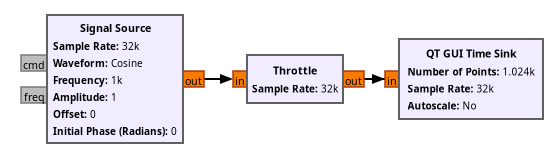
\includegraphics[width=0.5\linewidth]{gnu-dummy-bd.png}}\\[1PC]
    \subcaptionbox{GUI generada por GNU Radio.\label{fig::gnu-dummy-plot}}
    {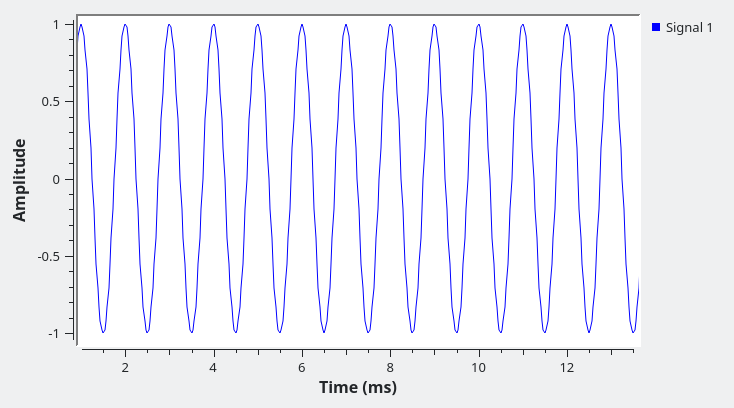
\includegraphics[width=0.5\linewidth]{gnu-dummy-plot.png}}
    \caption{Diagrama de bloques sencillo implementado en GNU Radio y la interfaz generada por el mismo.}
    \label{fig::gnu-dummy}
\end{figure}

\todo{Poner tabla con bloques nativos utilizados y otra con bloques custom o de otros usuarios (parecido a lo que hicimos con las IPs en el preproc)}

\section{Comprobación de algoritmos preexistentes}
Como primera instancia se evaluaron el algoritmo previamente implementado en \cite{proyecto-grigo} para realizar la estimación de DoA y la conformación digital de haz. Estos algoritmos se incorporó a GNU Radio en forma de bloque OOT, cuyas declaraciones y definiciones pueden encontrarse en el directorio \texttt{GNU-Radio/OOT/gr-beamforming/lib/}.

Para llevar a cabo la comprobación de funcionamiento de dichos bloques se generaron señales sintéticas mediante la utilización de \textit{Jupyter Notebook}, el generador se encuentra en \texttt{DOA/signal\_generator.ipynb}

Los desfases relativos para cada uno de los elementos $\Delta \varphi_{ij}$ viene dado por:
\begin{equation}
    \Delta \varphi_{ij} = k d \cos (\theta) \cdot (i \cos \phi + j \sin \phi),
    \label{eq::desfases}
\end{equation}
donde $\theta$ representa el ángulo de elevación y $\phi$ el de acimut, $k$ representa el número de onda y $d$ la separación entre elementos como se muestra en la figura \ref{fig::theta-phi}.

Dado que \[k =  \frac{2 \pi}{\lambda}\] y la separación entre elementos se eligió en el capítulo \todo{ref!} como \[d = 0.55\lambda,\] la ecuación \ref{eq::desfases} se simplifica a 
\begin{equation}
    \Delta \varphi_{ij} = 1.1 \pi \cos (\theta) \cdot (i \cos \phi + j \sin \phi).
    \label{eq::desfases-simplificada}
\end{equation}
Se ve entonces de la ecuación \ref{eq::desfases-simplificada} que, al elegir la separación entre elementos como un valor proporcional a la longitud de onda, los desfases asociados resultan independientes de la frecuencia.

Las señales generadas, de carácter complejo, fueron escritas a un archivo binario, el cual se leyó desde GNU Radio empleando el bloque \texttt{File Source}. Un detalle relevante en la configuración de este bloque es que deben saltearse los primeros 16 números complejos (los primeros 128~bytes) ya que corresponden al \textit{header} de los datos generados sintéticamente y no son de interés. 

Si bien no es necesario conocer el funcionamiento interno ni la implementación de estos bloques, si es necesario conocer su interfaz de entrada/salida para poder trabajar con ellos. En el caso del \texttt{DoA Esprit Estimation} recibe un vector complejo de tamaño $M_x \times M_y = 4 \times 4 = 16$ (ver figura \ref{fig::theta-phi}); por otro lado, a la salida se implementó un puerto de mensajes, el cual comunicará la dirección de arribo detectada al \texttt{Beamformer (C++)}. Este último recibe también un vector complejo de $M_x \times M_y = 4 \times 4 = 16$ elementos y su salida es un \textit{stream} de números complejos representando a la señal conformada. El bloque \texttt{File Source} puede configurarse para entregar un vector de 16 elementos complejos en cada lectura, que es exactamente lo que necesitan los bloques siendo evaluados.

Se probaron diversos valores tanto de acimut como de elevación y pudo conformarse la señal exitósamente utilizando el esquemático mostrado en la figura \ref{fig::doa-test}. En todos los casos logró detectarse correctamente la dirección de arribo y se realizó de manera exitosa la conformación de haz, verificando así el comportamiento de estos bloques.

\figura[0.7]{theta-phi}{Geometría de una arreglo rectangular uniforme. Para la generación de señales se tomo este modelo con $M_x = M_y = 4$\cite{proyecto-grigo}.}[Geometría de una arreglo rectangular uniforme.]

\figura[0.8]{doa-test}{Diagrama de bloques empleado para verificar el funcionamiento de los bloques \texttt{DoA Esprit Estimation} y \texttt{Beamformer (C++)}.}

\section{Desarrollo de algoritmos propios}
Se desarrollaron dos nuevos bloques OOT, uno de ellos es una reimplementación con algunas diferencias del \texttt{Beamformer (C++)} y el otro incorpora también la corrección del corrimiento Doppler. Su estructura y funcionamiento se detallan a continuación.

\subsection{Conformador de haz a partir de dirección de arribo}
Se reimplementó un nuevo bloque de conformación de haz ya que el preexistente fue diseñado para usarse exclusivamente en conjunto con \texttt{DoA Esprit Estimator}, dado que la única forma de comunicar la dirección de arribo es mediante el \texttt{doa\_port} como puede verse en la figura \ref{fig::doa-test}. 

Esto resulta impráctico cuando ya se conoce la dirección de arribo, como es el caso por ejemplo de las señales sintéticas. Para estas situaciones resultaría útil poder comunicar al conformador de haz la dirección de arribo de manera directa mediante la modificación de un parámetro. Con esto en mente se implementó un nuevo bloque OOT para conformar un haz a partir de una dirección de arribo configurada en los parámetros del bloque, el mismo puede encontrarse en \todo{Poner donde, ahora está en streaming on demand. Sacar de ahí y ponerlo en GNU Radio}. El esquemático empleado en la verificación de este bloque se muestra en la figura \ref{fig::bf-from-angles}.

\todo{Explicar el algoritmo de BF? Es basícamente revertir los defases de la ecuación \ref{eq::desfases-simplificada}}


\figura[0.9]{bf-from-angles}{Diagrama de bloques utilizado para la verificación del nuevo bloque conformador de haz.}

\subsection{Seguimiento y conformación de haz a partir de TLE}
El TLE codifica toda la información necesaria para describir la órbita de un satélite (ver apéndice \ref{ap::tle}), de manera que conociendo la ubicación de la estación terrena y la órbita de la misión objetivo es posible determinar la ubicación en el cielo de la misión respecto a la estación terrena, obteniendo así valores para los ángulos de elevación y acimut los cuales son necesarios para realizar la conformación de haz.

Más aún, con el TLE y la frecuencia de operación de la misión objetivo puede estimarse el corrimiento Doppler percibido desde la estación terrena. Luego, en base a esta estimación pueden incorporarse etapas de corrección del mismo.

Se desarrolló un módulo OOT de GNU Radio para el seguimiento de un satélite, la corrección del corrimiento Doppler y la conformación digital de haz.

\subsubsection{La librería \textit{orbit-predictor}}
Para la implementación de este bloque se hizo uso de las funciones provistas en la librería \textit{orbit-predictor} de Python desarrollada en un repositorio de GitHub de Satellogic~\cite{orbit-predictor}. Esta librería incluye numerosas funciones relacionadas a la predicción de órbitas. De interés resulta la posibilidad de introducir el TLE como parámetro para el predictor de órbita de un satélite.

La librería cuenta con objetos de tipo \texttt{Location} que representan un punto en el planeta Tierra mediante la especificación de latitud, longitud y altura. Se definió un nuevo objeto \texttt{Location} ubicado en las coordenadas de la futura instalación de la estación terrena, las cuales se detallan en la tabla \ref{tab::coords-et}.

\begin{table}[H]
\centering
\resizebox{0.5\textwidth}{!}{%
\begin{tabular}{|ll|}
\hline
\multicolumn{2}{|l|}{\textbf{Coordenadas utilizadas para la estación terrena}} \\ \hline
\multicolumn{1}{|l|}{Latitud {[}$\degree${]}} & -41.123 \\ \hline
\multicolumn{1}{|l|}{Longitud {[}$\degree${]}} & -71.410 \\ \hline
\multicolumn{1}{|l|}{Altura {[}msnm{]}} & 769 \\ \hline
\end{tabular}%
}
\caption{Ubicación de la estación terrena considerada para realizar los cálculos.}\label{tab::coords-et}
\end{table}


Se implementaron además tres funciones para las siguientes tareas:
\change{Chequear si hice esto así o si mejor lo digo en el streaming on demand}
\begin{itemize}
    \item Calcular la próxima pasada del satélite por la estación terrena. La librería permite además la configuración de un ángulo de elevación mínimo a patir del cual considerar que comienza la pasada.Se configuró el comienzo de una pasada cuando el satélite se encuentra a $10\degree$ sobre el horizonte ($\theta = 10\degree$).
    \item Obtener y actualizar los ángulos de conformación de haz en base al cálculo de la ubicación del satélite en el cielo respecto a la estación terrena.
    \item Calcular  y actualizar el factor de corrimiento Doppler respecto a la ubicación de la estación terrena.
\end{itemize}


\figura[0.9]{bf-from-tle}{Diagrama de bloques que utiliza los TLE para realizar el seguimiento de la misión, la corrección del corrimiento Doppler y la conformación de haz.}


\subsection{Pruebas en capturas reales}
Se comprobó el funcionamiento de los algoritmos tanto preexistentes como el nuevo algoritmo de \textit{beamforming} mediante la lectura de capturas reales adquiridas en \cite{proyecto-jose} con el emulador de arreglo de 16 canales realizado en ese mismo proyecto.

La integración de estas capturas con los bloques de conformación de haz disponibles no es directa ya que las mismas contienen la información de cada canal codificada como enteros de 16 bits (\textit{shorts}), los cuales fueron escritos en formato \textit{offset binary} \todo{ref de qué es off bin}, \unsure{Realmente vale la pena explicar esto?}

\todo{Capaz poner una tabla con señales generadas (angulos) vs angulos detectados}

\figura{signal-complexer2}{Complejizador}





\subsection{Comunicación entre CIAA-ACC y GNU Radio}\label{subsec::comuicacion-con-gnuradio}
Se mencionó anteriormente que el sistema de adquisición y preprocesamiento envía paquetes con los datos adquiridos mediante un socket UDP. Luego, del lado de GNU Radio, esos paquetes deben capturarse e interpretarse correctamente. 

La captura de los paquetes puede lograrse a través de la instanciación del bloque \texttt{UDP Source}\todo{ref}, disponible con la instalación de la librería. Este bloque escucha el tráfico UDP entrante a un dado puerto y proveniente de una dirección IP \unsure{Acá IP es Internet Protocol, no es Intellectual Property, cómo se resuelve esto?} determinada. De esta forma, configurándolo con la dirección IP de la CIAA-ACC y el número de puerto al que la placa transmite, pueden recibirse los datos exitósamente en GNU Radio. 

Al configurar el bloque \texttt{UDP Source} también hay que especificarle el tamaño de paquete que esperamos recibir. Resulta importante notar que, a diferencia de la mayoría de los bloques de la librería, dicho tamaño se escribe siempre en bytes, independientemente del tipo de dato con el que se esté trabajando.

Por otro lado, para lograr una correcta interpretación de los datos debe tenerse en cuenta el tipo de dato que se está adquiriendo. El sistema de tipado de la librería se desarrolla en el apéndice \ref{ap::tipado-gnu}. En el caso de este proyecto, los datos que llegan desde el sistema de adquisición y preprocesamiento son complejos, donde la parte real y la imaginaria se componen de 16 bits cada una. \todo{ref} El bloque \texttt{UDP Source}, sin embargo, no es capaz, por defecto, de entregar los datos en este formato, ya que el tipo complejo con el que trabaja (\texttt{Complex Float 32}) se compone de 64 bits en total.

Una solución a este problema es leer los datos de a 16 bits y luego agrupar dos datos de 16 bits como un único dato complejo de 32 bits. Esto se logra configurando el tipo de dato del \texttt{UDP Source} como \texttt{short}, que es un entero de 16 bits. Luego mediante la instanciación del bloque \texttt{IShort To Complex}, el cual forma parte de la librería, se convierten dos \texttt{shorts} consecutivos en un \texttt{Complex Float 32}. De esta manera, se puede trabajar durante todo el procesamiento con datos del tipo \texttt{Complex Float 32}.

\subsubsection{Composición del paquete}
Desde el lado del software desarrollado en \cite{proyecto-jose} se fijó una estructura del paquete de datos adquirido, el cual se ilustra en la figura \ref{fig::paquete-original}. Dicho paquete se compone de 87~bytes de \textit{header} y su \textit{payload} consiste de 1000~muestras de cada uno de los 16~canales del ADC escritas de manera secuencial, esto es: 1000~muestras del primer canal, seguidas de 1000~muestras del segundo canal y así sucesivamente.

Esta estructura resulta incómoda para interactuar con GNU Radio por dos motivos:
\begin{enumerate}
    \item Dado que se concluyó que los datos se interpretaran como datos de tipo \texttt{short}, los mismos se agruparan de a 2~bytes. Luego, el \textit{header}, al ser un mútiplo de 2~bytes, no puede separarse con facilidad.
    
    \item El hecho de que las muestras de los canales vengan agrupadas por canal dificulta la demultiplexación de los datos. Más sencillo sería si se agrupáse por número de muestra, enviando la primera muestra de cada uno de los 16 canales, seguida por la segunda muestra de cada uno de los 16 canales y así sucesivamente.
\end{enumerate}

Se realizaron entonces dos cambios fundamentales para facilitar la comunicación con GNU Radio. Por un lado se realizó un \textit{padding} de 1~byte del \textit{header} para que tenga un largo par (88~bytes). Por otro lado, se modificó la estructura mostrada en la figura \ref{fig::paquete-original} para lograr la estructura de intercalación de canales por número de muestra descrita en el punto 2.

Finalmente, el largo total del paquete resulta \[88\un{bytes} + 16\un{canales} \times 4\un{bytes/muestra/canal} \times 1000\un{muestras} = 64088\un{bytes}.\]

\figura[0.5]{paquete-original}{Paquete de datos adquirido original desarrollado en \cite{proyecto-jose}.}[Paquete de datos adquirido original.]

\todo{foto nueva estructura}

\subsection{Lector de \textit{header}}
Como se mencionó, el paquete enviado por la placa incorpora un \textit{header}. El mismo fue desarrollado en \cite{proyecto-jose} y su estructura puede encontrarse en \texttt{PIQuinteros/SoftwarePS/client/lib/acqPack.h}.

Este encabezado consiste de 88 bytes y contiene, entre otras cosas, las \textit{fifo flags} (ver figura \ref{fig::paquete-original}). Estas son señales de control que permiten el monitoreo de las FIFOs dentro de la FPGA. Resultan relevantes para detectar por ejemplo situaciones de \textit{overflow}, lo cual puede ocurrir si las FIFOs se llenan antes de ser leídas por el PS.

Para poder decodificar el encabezado de los paquetes se implementó un módulo OOT personalizado en GNU Radio empleando la herramienta \textit{gr\_modtool} mencionada anteriormente. La definición del mismo se encuentra en \texttt{GNU-Radio/OOT/gr-beamforming/lib/HeaderReader\_impl.h}. 

El bloque recibe un vector del tamaño del \textit{header} (88 bytes) y lo decodifica. A continuación verifica que la información relevante durante ejecución como la \textit{flag} de \textit{FIFO overflow} y la \textit{flag} de \textit{FIFO full} sea la adecuada y, en caso contrario, avisa al usuario escribiéndolo a la consola integrada de GNU Radio.

\todo{Poner foto del header o referencia si es que lo expliqué antes. Ver pag 70 del informe de José}

\subsection{Comprobación de funcionamiento}
Para corroborar que la comunicación entre la placa y el SDR estaba funcionando de manera correcta se configuró la FPGA para obtener datos del contador de debug mediante la escritura de los registros \todo{decir registros, poner ref a cuando se explicó}. A continuación se disparó una captura de datos, la cual se adquirió con GNU Radio.

En la figura \ref{fig::gnu-simplificado} se muestra el esquemático utilizado para esta comprobación. El mismo incorpora lo anteriormente discutido junto con dos puntos de visualización donde se colocaron instancias del bloque \texttt{QT GUI Sink}, el cual brinda, entre otras cosas un gráfico en tiempo y en frecuencia de la señal de entrada.

Se separaron los datos en \textit{header} y \textit{payload} mediante el uso del bloque \texttt{Stream Demux}. Como se mencionó, el tamaño total del paquete resulta de 64088~bytes, de los cuales los primeros 88 corresponden al \textit{header} y el resto corresponde al \textit{payload}. Al interpretar los datos como \texttt{shorts}, debe configurarse el \texttt{Stream Demux} para enviar los primeros 32000~\texttt{shorts} por un puerto y los otros 44 por el otro.

Se disparó luego una captura desde la placa utilizando datos del contador mencionado en la tabla \ref{tab::fifo-input-mux}. El uso de un contador permite de manera sencilla identificar pérdida de datos. Se observó que se recibían los datos de todos los canales y se comprobó el correcto funcionamiento del contador y la interfaz de comunicación, esto se muestra en la figura \ref{fig::grafico-contador}. Allí se muestra la señal recibida en todos los canales, esto es, antes del \texttt{Stream Demux} complejo mostrado en la figura \ref{fig::gnu-simplificado}. Se observa que todos los canales reciben el mismo valor del contador, y que este último avanza de uno en uno como se esperaba.

Se procedió a continuación a la captura de datos crudos del oscilador local de \textit{debug} desarrollado en el capítulo \ref{cap::preproc}. Con la frecuencia del mismo configurada a $19.51\un{MHz}$, se adquirió un único paquete para evitar el \textit{overflow} en las FIFOs y se verificó que se recibía un tono real a esa frecuencia, como se muestra en la figura \ref{fig::grafico-raw-local-osc}.

Como siguiente paso, se configuró el registro que controla el \texttt{FIFO Input Mux} para visualizar la salida de datos del preprocesamiento. Con la señal del oscilador local de \textit{debug} se espera encontrar a la salida del preprocesamiento un tono complejo centrado en $-10\un{kHz}$ como se obtuvo cuando se simuló con UVM en la sección \ref{sec::simu-uvm}. En la figura \ref{fig::grafico-preproc} se muestra la salida del preprocesamiento, donde efectivamente se ve dicho tono y se observa también \textit{aliasing}, habiendo un tono indeseado en 10~kHz. Este \textit{alias}, sin embargo, se encuentra más de 40~dB por debajo del tono de $-10\un{kHz}$. Esta atenuación concuerda con la fijada para el filtro de haz en la tabla \ref{tab::filtro-beam-nuevo}.

Por último, para verificar el correcto funcionamiento del \texttt{Header Reader} se adquirieron datos crudos (generados a 65~MSps) con el objetivo de intencionalmente provocar \textit{overflow} en las FIFOs para verificar si esto era debidamente decodificado y notificado al usuario. Se comprobó este comportamiento de manera exitosa, obteniendose mensajes de \textit{overflow} en la consola.

\figura{gnu-simplificado}{Esquemático utilizado para la prueba de comunicación entre la CIAA-ACC y GNU Radio.}

\figura[0.6]{grafico-contador}{Gráfico de la señal detectada en todos los canales juntos (antes del \texttt{Stream Demux} complejo) en función del tiempo.}

\figura[0.6]{grafico-raw-local-osc}{Gráfico de la ganancia relativa en función de las componentes de frecuencia de la señal cuando la entrada son los datos crudos del oscilador local de \textit{debug}.}

\figura[0.7]{grafico-preproc}{Gráfico de la ganancia relativa en función de las componentes de frecuencia de la señal cuando la entrada son los datos preprocesados.}

\section{Validación de la cadena de adquisición y procesamiento}
A lo largo del desarrollo del sistema de adquisición y preprocesamiento en el capítulo \ref{cap::preproc} se validaron las etapas de manera aislada. De igual manera, en el desarrollo de la etapa de procesamiento externo se comprobó el funcionamiento del conformador de haz, la detección de dirección de arribo y la lectura de \textit{header} de manera individual.

Resulta igualmente importante para la validación del sistema la realización de pruebas de integración o \textit{integration tests}. Para esto se hizo uso de un sistema de emulación de un arreglo lineal de 4 elementos desarrollado en \cite{proyecto-arce}.

En dicho proyecto se programó un microcontrolador STM32F1\cite{stm32f1} para generar señales que emulen las señales recibidas por un arreglo lineal de 4 antenas. Estas señales en principio digitales, pasan a través de un DAC y se emiten de manera analógica empleando el integrado AD9959\cite{ad9959}. 

Las señales de salida del integrado entonces emulan la recepción de señales resultantes de la pasada de un satélite, la implementación realizada en~\cite{proyecto-arce} tiene parámetros ajustables, estos son:
\begin{itemize}
    \item Altura del satélite.
    \item Frecuencia central.
    \item Distancia entre elementos.
\end{itemize}

\todo{Mencionar que también se emula el corrimiento Doppler}

\subsection{Adaptación del emulador}\label{subsec::adaptacion-emulador}
El emulador original replica un arreglo lineal de $4 \times 1$ elementos que solo emula variaciones en el ángulo de elevación $\theta$, sin embargo, para que el bloque \texttt{DoA Esprit Estimation} funcione, este debe recibir señales de un arreglo cuadrado. Por esto es necesario refactorizar el código desarrollado en \cite{proyecto-arce} para emular un arreglo cuadrado de $2 \times 2$ elementos.

Para esto, si se desea mantener únicamente un parámetro variable (el ángulo de elevación), puede enviarse la misma señal a dos antenas adyacentes y una señal desfasada a las dos antenas restantes. De esta manera, el arreglo de $2 \times 2$ solo recibe variaciones en $\theta$ y se corresponde al caso donde la pasada del satélite es perpendicular al arreglo, esto se corresponde con el conjunto de ángulos de acimut $\phi:$~$[0\degree, 90\degree, 180\degree, 270\degree]$, dependiendo de cuáles dos antenas reciben la misma señal. El diagrama de bloques empleado para esta comprobación se muestra en la figura \ref{fig::bd-array-2-2}.

\figura[1]{bd-array-2-2}{Diagrama de bloques utilizado para la adaptación del arreglo, la detección de dirección de arribo y la conformación de haz.}
\todo{Continuar, alguna foto}

\subsection{Extensión a 16 canales}\label{subsec::ext-16-canales}
Durante la operación del receptor, el software deberá lidiar con 16 canales en simultáneo. Para verificar la capacidad del mismo para hacerlo, partiendo del arreglo lineal de $4 \times 1$, se replicó la señal de cada antena cuatro veces, de manera de obtener un arreglo de $4 \times 4$ análogo al arreglo de $2 \times 2$ obtenido en la subsección \ref{subsec::adaptacion-emulador}, donde el ángulo de acimut puede tomar los siguientes valores $\phi = [0\degree, 90\degree, 180\degree, 270\degree]$. El diagrama de bloques empleado para esta comprobación se muestra en la figura \ref{fig::bd-array-4-4}.

\figura[1]{bd-array-4-4}{Diagrama de bloques utilizado para la simulación del arreglo de $4 \times 4$ elementos.}

\subsection{Incorporación del ángulo de acimut}

\subsection{Pruebas con un segundo emulador de arreglo}
Las pruebas realizadas con el emulador de arreglo lineal desarrollado en \cite{proyecto-arce} permitieron validar gran parte del sistema como se desarrollo en las subsecciones anteriores. No obstante, solo genera 4 señales, de manera que no permite validar los 16 canales del ADC operando en simultáneo. Se hizo una extensión a 16 canales en la subsección \ref{subsec::ext-16-canales}, pero esta extensión se realiza en software, no en hardware.

Para poder realizar una prueba que utilice los 16 canales físicos del ADC se hizo uso del emulador de arreglo desarrollado y fabricado en \cite{proyecto-jose}. El mismo es un emulador de un arreglo de $4 \times 4$ elementos dispuestos de forma rectangular y separados una distancia $\lambda/2$, donde $\lambda = \frac{c}{146\un{MHz} \approx 2.05\un{m}}$. Resulta relevante notar que este emulador no fue hecho para la banda de UHF en la que opera el receptor desarrollado en este proyecto, sino para la banda de VHF de 144~MHz a 148~MHz.

No obstante, pueden configurarse las frecuencias de los osciladores dentro de la placa para poder preprocesar señales en esta banda.

Una señal de entrada a $147\un{MHz}$, por ejemplo, se \textit{mapea} a \[147\un{MHz} - 2 \times 65 = 17\un{MHz}\] tras el muestreo pasabanda. Luego, la rotación de espectro de $18.5\un{MHz}$ causado por la mezcla de banda traslada el tono a $1.5\un{MHz}$, dejándolo en el límite de la banda de paso. Finalmente, configurando el oscilador de haz para operar a $-1.5\un{MHz}$ se obtiene la señal en banda base.

Este emulador, a diferencia del utilizado en las demás comprobaciones, emula la recepción de una señal inmóvil desde una dirección fija, lo cual no permite comprobar las capacidades del sistema de realizar un seguimiento de la señal. Estas capacidades, sin embargo, ya fueron evaluadas en las anteriores subsecciones.

\todo{fotos}

\end{document}